\documentclass{standalone}

\usepackage{tikz,pgf}
\usetikzlibrary{arrows}

\begin{document}
	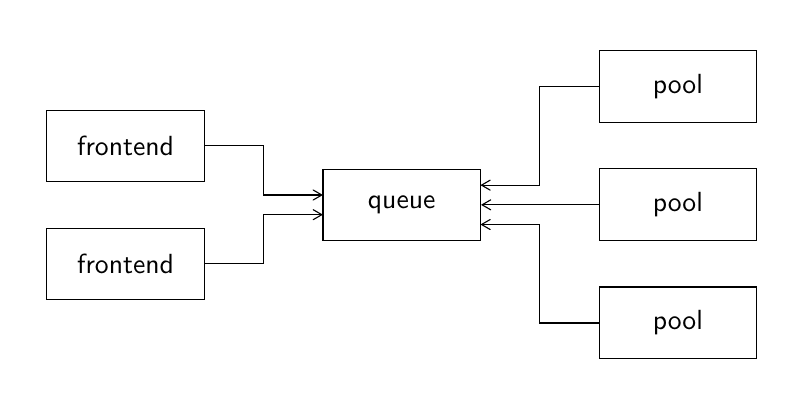
\begin{tikzpicture}[font=\sf,component/.style={draw,shape=rectangle, inner sep=3mm,minimum width=2cm,minimum height=0.9cm}]
		\useasboundingbox (-4.75,2.25) rectangle (4.75,-2.25);
		%%%
		\node[component] (queue) at (0,0) {queue};
		\node[component,anchor=west] (poolA) at (2.5,1.5) {pool};
		\node[component,anchor=west] (poolB) at (2.5,0) {pool};
		\node[component,anchor=west] (poolC) at (2.5,-1.5) {pool};
		\node[component,anchor=east] (frontendA) at (-2.5,0.75) {frontend};
		\node[component,anchor=east] (frontendB) at (-2.5,-0.75) {frontend};
		%%%
		\draw[angle 60-] (queue) -- (poolB);
		\draw[angle 60-] (1,0.25) -- (1.75,0.25) |- (poolA);
		\draw[angle 60-] (1,-0.25) -- (1.75,-0.25) |- (poolC);
		\draw[-angle 60] (frontendA) -- (-1.75,0.75) |- (-1,0.125);
		\draw[-angle 60] (frontendB) -- (-1.75,-0.75) |- (-1,-0.125);
	\end{tikzpicture}
\end{document}